\section{Basics}\label{sec_basics}
    PEC takes advantage of the photovoltaic\index{photovoltaic} effect, discovered by 
    \citet{becquerel1839} in 1839, that occurs at the interface of a semiconductor
    and an electrolyte. 
    In fact, the first experience showed the occurrence of a photopotential and 
    a photocurrent under illumination when a silver electrode, 
    covered with an oxide layer, was immersed in an acidic medium and connected 
    to a platinum electrode. 
    Nonetheless, the first studies focused on the understanding of the interfacial 
    processes were performed much later 
    \citep{stimming1986,gerischer1966,copeland1942}.

    The basics of photoelectrochemistry and application examples are presented in 
    the following sections and they are largely described in the literature 
    \citep{morrison1980,gerischer1985,memming2008,marcus2006,bard2002,sato1998}. 
    Several hypotheses are needed in order to apply the theoretical concepts:  
    \begin{itemize}
        \item semiconductor are considered to be ideal i.e. crystallized and homogeneous  
        \item the dielectric constant of the semiconductor is independent of the light wavelength  
        \item the capacity of the Helmholtz layer is greater than the capacitance of the space charge capacitance  
        \item the potential drop in the Helmholtz layer is independent of the applied potential and is negligible
    \end{itemize}

    The hypotheses are rarely fully respected in the case of oxides or passive 
    films formed on industrial alloys. Nonetheless, the literature shows that the 
    developed models can be applied to non-ideal systems such as oxides 
    and passive films.


\subsection{Electronic Band Structure}
    Solids are generally classified into three groups: 
    conductors\index{conductors}, semiconductors\index{semiconductors} and isolators\index{isolators}. 
    Each category can be illustrated with a specific band structure as shown in 
    figure~\ref{fig_band_model}. 
    Valence\index{band!valence} and conduction\index{band!conduction} bands correspond to allowed energy states for the electrons. 
    The lowest energy level of the conduction band is labeled $E_c$ and the 
    highest energy level of the valence band is labeled $E_v$. 
    They are separated by a band gap\index{bandgap}, $E_g$, with no allowed energy states. 
    The repartition of the electrons among both bands are described by the position 
    of the Fermi Level\index{Fermi!level}, $E_F$, which represents the highest energy state that 
    can be occupied level at 0K. 
    It is equivalent to the electrochemical potential\index{potential!electrochemical} in solid phases.

    \begin{figure}[h]
        \centering
            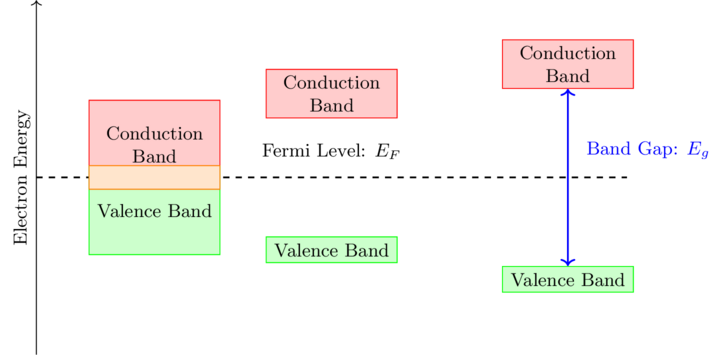
\includegraphics[width=0.85\textwidth]{tikz_band_model.png}
        \caption{Schematic representation of the electronic band structure \citep{marucco2006}: 
        a) conductor, b) semiconductor, c) insulator}
        \label{fig_band_model}
    \end{figure}

    The electronic conduction\index{conduction!electronic} is due to the movement either of the negatively 
    charged electrons in the conduction band or of the positively charged holes 
    in the valence band or both simultaneously. 
    Consequently, the conduction depends on the number of available charge carriers
    in the conduction band\index{band!conduction} and in the valence band\index{band!valence}. 
    In conductors, an overlap of the conduction and the valence bands occurs 
    which means that the highest allowed energy band is partially filled. 
    The distinction between a semiconductor and an insulator is less obvious 
    because the conduction depends on the band gap and the energy provided by 
    the environment to the electrons from the valence band in order to jump 
    into the conduction band.

    In semiconductors, charge carriers can be generated by three mechanisms: 
    \emph{thermal excitation, photoexcitation and doping} as shown in 
    figure~\ref{fig_excitation_carrier}. \index{thermal excitation} \index{photoexcitation}, \index{doping}
    In the case of very low band gaps, thermal excitation can be enough in order 
    to eject an electron from the valence band to the conduction band. 
    Photoexcitation ejects electrons from the valence band to the conduction 
    band when an incident photon, with energy greater than the band gap, is absorbed. 
    Doping introduces additional energy level located in between the conduction and 
    valence bands.

    Doping occurs when the stoichiometry is altered or when impurities are 
    introduced in the crystallographic lattice of the semiconductor. 
    In the case of n-type semiconductors, the donor energy levels $E_d$ lie just 
    under the conduction band. The electrons from the donor levels are ejected by 
    thermal excitation. 
    Consequently, the majority charge carriers are negatively charged electrons 
    in the band conduction. 
    Similarly, the acceptor energy levels $E_a$, of p-type semiconductors, 
    lie just above the band valence. 
    The latter trap electrons from the valence band and therefore create holes. 
    Consequently, the majority charge carriers are positively charged holes.

    \begin{figure}[h]
        \centering
        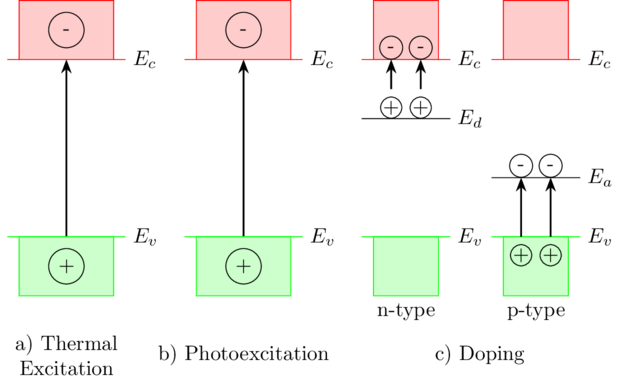
\includegraphics[width=0.85\textwidth]{tikz_excitation_carrier.png}
        \caption{Schematic representation of the mechanisms generating charge carriers in semiconductors \citep{finklea1983}: 
        a) thermal excitation, b) photoexcitation, c) doping}
        \label{fig_excitation_carrier}
    \end{figure}

    The Fermi level $E_F$ in intrinsic semiconductors is located at the mid-gap \index{Fermi!mid-gap}. 
    The n-type and p-type doping\index{doping!n-type}\index{doping!p-type} shift the Fermi level towards band edges 
    $E_c$ and $E_v$, respectively. \index{Fermi!shift}
    The figure~\ref{fig_fermi_position} shows the position of the Fermi level 
    with respect to the semiconductor type. \index{Fermi!position}

    \begin{figure}[H]
        \centering
        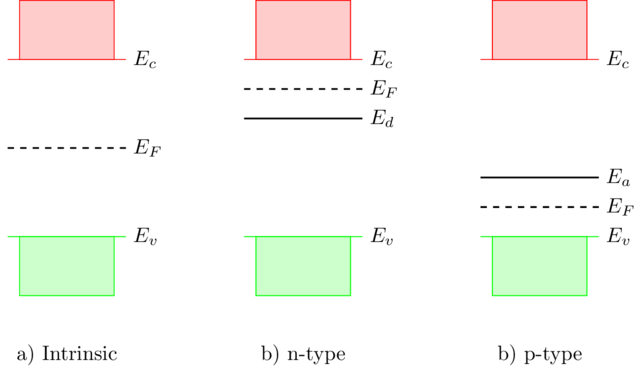
\includegraphics[width=0.85\textwidth]{tikz_fermi_position.png}
        \caption{Schematic representation of the Fermi level with respect to the 
        semiconduction type \citep{finklea1983}: a) intrinsic, b) n-type, c) p-type.}
        \label{fig_fermi_position}
    \end{figure}



\subsection{Semiconductor/electrolyte interface in dark condition}
    A potential gradient occurs when a semiconductor comes into contact with an 
    electrolyte as shown in figure~\ref{fig_interface_potential}.
    The position of the Fermi level\index{Fermi!level} in the electrolyte with respect to the 
    conduction and valence band edges leads to three different situations after 
    a transient charge transfer. \index{band!conduction}\index{band!valence}
    The flat band situation occurs when the Fermi level in the electrolyte 
    matches the Fermi level in the semiconductor. \index{Fermi!level} 
    Consequently, there is no potential gradient in the semiconductor. 
    In a case of Fermi level mismatch, a band bending occurs in the semiconductor 
    near the semiconductor/electrolyte interface.  \index{band!bending}
    The band bending leads to either depletion or accumulation of majority 
    charge carriers near the semiconductor/electrolyte interface. 
    The spatial extension of the depletion/accumulation zone is called space 
    charge as shown in figure~\ref{fig_space_charge_depletion}. \index{space charge}

    \begin{figure}[h]
        \centering
        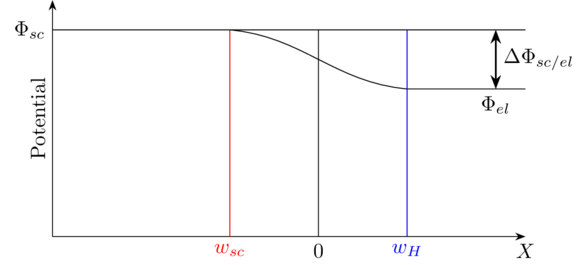
\includegraphics[width=0.85\textwidth]{tikz_interface_potential.png}
        \caption{Potential gradient at semiconductor/electrolyte interface 
        \citep{marcus2006}. $\Phi_{sc}$ and $\Phi_{el}$ correspond to the 
        potentials of the semiconductor and the electrolyte, respectively. 
        $\Delta Phi _{sc/el}$ corresponds to the potential difference between 
        the semiconductor and the electrolyte. $w_{sc}$ and $w_{H}$ correspond to 
        the widths of the space charge and the electrical double layer, 
        respectively.}
        \label{fig_interface_potential}
    \end{figure}

    \begin{figure}[H]
        \centering
        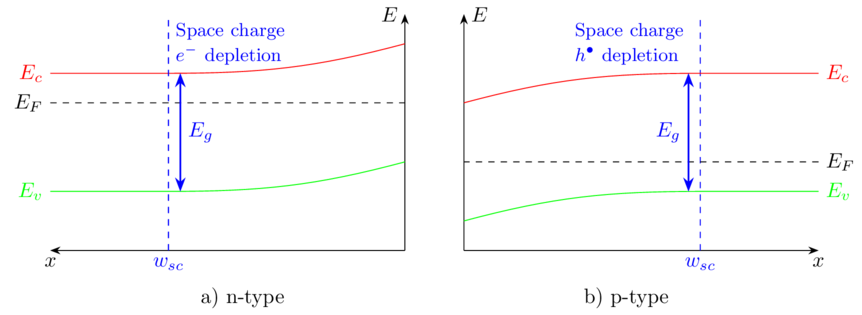
\includegraphics[width=0.85\textwidth]{tikz_space_charge_depletion.png}
        \caption{Schematic representation of the space charge in depletion of majority charge carriers for 
        a semiconductor in contact with an electrolyte \citep{memming2008,bard2002}:
         a) n-type, b) p-type.}
        \label{fig_space_charge_depletion}
    \end{figure}

    Depletion and accumulation as well as band bending can be obtained 
    by polarizing the semiconductor. \index{accumulation}\index{depletion}
    As long as the hypothesis described in the introduction paragraph stand, 
    the polarization does not modify the surface band edges $E_{cs}$ and $E_{vs}$. 
    Consequently, the polarization will only alter the band bending in the space 
    charge. 
    Depending on the applied potential, $U$, with respect to the flat band 
    potential, $U_fb$, three different situations will occur as shown in 
    figure~\ref{fig_band_bending}\index{potential!flat band}:
    \begin{itemize}
    \item $U = U_{fb}$: flat band situation no matter the semiconductor type
    \item $U > U_{fb}$: depletion (accumulation) in a case of n-type (p-type) semiconductor  
    \item $U < U_{fb}$: accumulation (depletion) in a case of n-type (p-type) semiconductor
    \end{itemize}

    Without illumination, cathodic (anodic) currents are favored in a case of 
    accumulation of electrons (holes) for an n-type (p-type) semiconductor. 
    In fact, the majority charge carriers of n-type (p-type) semiconductors are 
    electrons (holes). \index{illumination}
    Reciprocally, anodic (cathodic) currents are not favored in a case of 
    depletion of electrons (holes) for an n-type (p-type) semiconductor. 
    The junction between a semiconductor and an electrolyte acts like a Schottky diode.
    \index{junction}\index{Schottky}

    \begin{figure}[H]
        \centering
            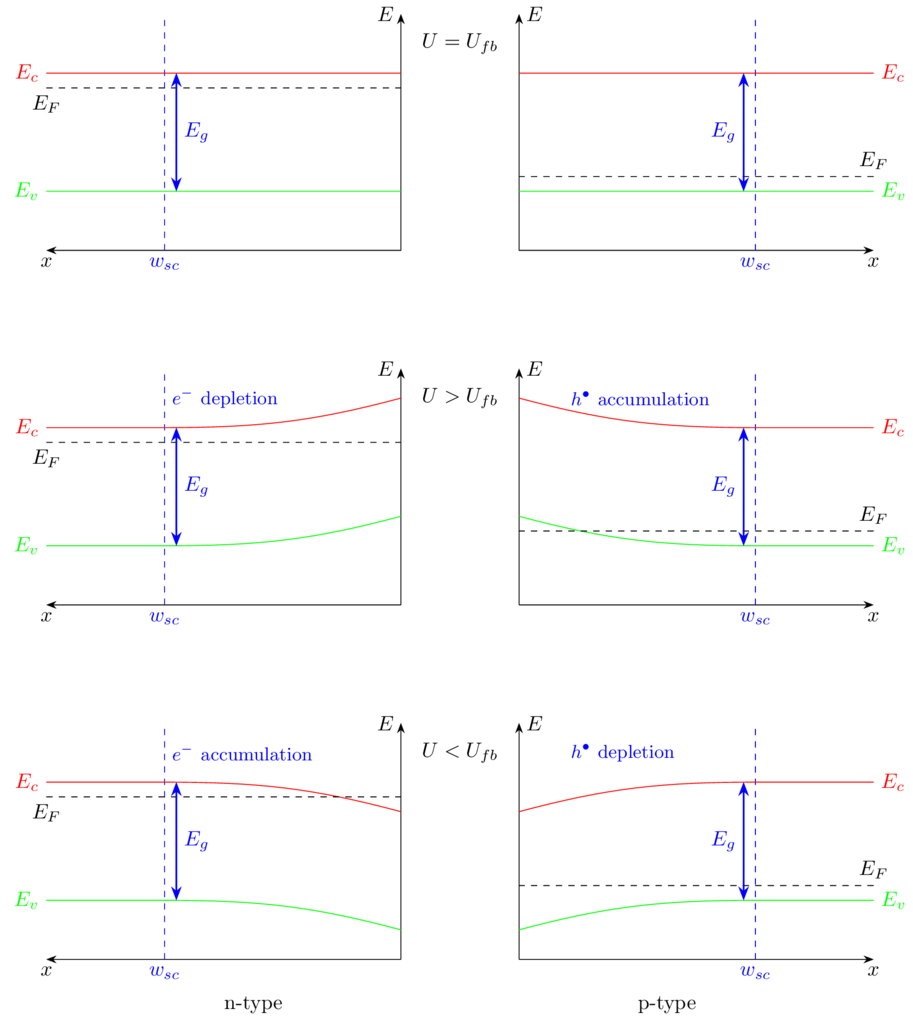
\includegraphics[width=0.85\textwidth]{tikz_band_bending.png}
        \caption{Schematic representation of the band bending in p-type and n-type 
        semiconductors in contact with an electrolyte \citep{memming2008, bard2002}:
         a) $U = U_{fb}$, b) $U > U_{fb}$, c) $U < U_{fb}$.}
        \label{fig_band_bending}
    \end{figure}
    \clearpage


\subsection{Semiconductor/electrolyte interface under illumination}
    The illumination of the semiconductor/electrolyte interface, 
    with photons having an energy greater than the band gap, $E_g$, creates 
    electron/hole pairs in the semiconductor. \index{band!gap}
    By applying the adequate potential the pairs can be separated. 
    As a consequence, the majority charge carriers are attracted to the 
    semiconductor bulk whereas the minority charge carriers are drawn to the 
    semiconductor/electrolyte interface where they can be transferred to a RedOx 
    species creating an additional current called photocurrent. \index{photocurrent} 

    Figure~\ref{fig_photocurrent_generation} illustrates schematically the 
    mechanism leading to the creation of a photocurrent. n-type (p-type) 
    semiconductors generate anodic (cathodic) photocurrents where the 
    electrons (holes) move towards the external circuit whereas the holes (electrons) 
    move towards the interface. 
    The photocurrent is significant when the semiconductor/electrolyte junction 
    is in depletion. 
    Figure~\ref{fig_photocurrent_plieth} shows the anodic (cathodic) photocurrent 
    for a GaAs n-type (p-type) semiconductor.

    Therefore, the applied potential on n-type (p-type) semiconductors is 
    greater (lower) than the flat band potential. \index{potential!flat band}

    \begin{figure}[h]
        \centering
        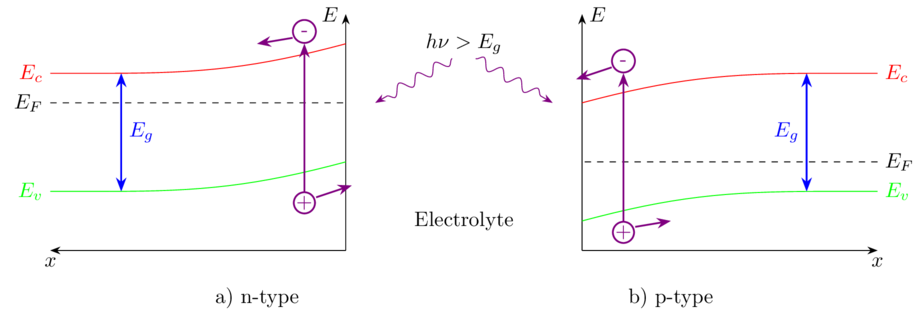
\includegraphics[width=0.85\textwidth]{tikz_photocurrent_generation.png}
        \caption{Schematic representation of the mechanism generating 
        a photocurrent \citep{memming2008,bard2002}.}
        \label{fig_photocurrent_generation}
    \end{figure}

    \begin{figure}[h]
        \centering
        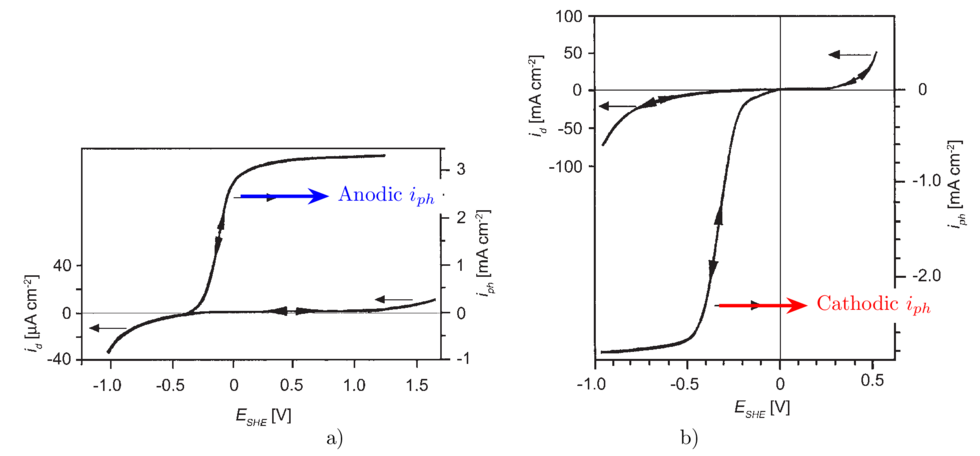
\includegraphics[width=0.85\textwidth]{tikz_photocurrent_plieth.png}
        \caption{Photocurrent density $i_{ph}$ and dark current density 
        $i_d$ with respect to the potential in a case of GaAs semiconductor 
        \citep{plieth2008}: a) n-type, b) p-type.}
        \label{fig_photocurrent_plieth}
    \end{figure}

    \citet{gartner1959} and \citet{butler1977} \index{Gärtner-Butler!model} 
    proposed a simple and robust model for 
    describing the photocurrent considering that the recombination of the 
    photogenerated electron/hole pairs does not occur in the space charge. \index{space charge}
    Therefore, the photocurrent is proportional to the photon flux $\Phi _0$. 
    Moreover, the photocurrent depends on the relative ratio between the space 
    charge width, $w_{sc}$, the depth of photon penetration given by the inverse 
    of the absorption coefficient, $ \alpha $, and the average diffusion length, 
    $L_{cc}$, of the minority charge carriers. 
    In other words, all absorbed photons generate electron/hole pairs and 
    the minority charge carriers are transferred to the electrolyte and 
    therefore contribute to the photocurrent whose expression is given 
    by the equation~\ref{eq_iph_gartner_butler}.

    \begin{equation}
        I_{ph} = \phi _0 \left[ 1 - \frac{\exp (-\alpha _{sc} \cdot w_{sc})}{1+\alpha _{sc} \cdot
        L_{cc}} \right]
        \label{eq_iph_gartner_butler}
    \end{equation}

    When $\alpha _{sc} \cdot w_{sc} \ll 1$ and $\alpha _{\sc} \cdot L_{cc} \ll 1$, 
    the photocurrent is approximated by the 
    equation~\ref{eq_iph_gartner_butler_simplified}.

    \begin{equation}
        I_{ph} = \phi _0 \cdot \alpha _{\sc} \cdot w_{sc}
        \label{eq_iph_gartner_butler_simplified}
    \end{equation}

    The expression of the space charge width, $w_{sc}$, in depletion is given 
    by the equation~\ref{eq_space_charge_Schottky} according to the Mott-Schottky theory.\index{mott-schottky} 
    $N_{cc}$ represents the number of majority charge carriers, supposed to be 
    equal to the doping, $e$ corresponds to the elementary charge of an electron., 
    $U$ represents the applied potential, $U_{fb}$ represent the flat band 
    otential, $\epsilon$ and $\epsilon _0$ represent the relative and the 
    vacuum permittivity, respectively. \index{potential!flat band} \index{space charge} \index{depletion}

    \begin{equation}
        w_{sc} = \sqrt{ \frac{2\epsilon \epsilon _0}{e N_{cc}} (U-U_{fb}-\frac{kT}{e}) }
        \label{eq_space_charge_Schottky}
    \end{equation}

    The expression of the absorption coefficient $\alpha _{sc}$ with respect to 
    the light energy $h\nu$ is shown in equation~\ref{eq_absorption_coef}. 
    The value of $n$ depends on the band-band transition type. $n$ takes discreet 
    values of 0.5 or 2 when direct or indirect transitions are allowed, respectively.
    \index{coefficient!absorption} \index{transitions!direct} \index{transitions!indirect}

    \begin{equation}
        \alpha _{sc} = const \frac{(h\nu - E_g)^n}{h\nu}
        \label{eq_absorption_coef}
    \end{equation}

    The complete expression of the photocurrent is therefore given by the 
    equation~\ref{eq_iph_substitute_W_alpha}. 
    The latter is obtained by substituting the absorption coefficient $\alpha _{sc}$ 
    and the space charge width $w_{sc}$ from the 
    equation~\ref{eq_iph_gartner_butler_simplified}
    by the equations~\ref{eq_space_charge_Schottky} and \ref{eq_absorption_coef}, 
    respectively. \index{photocurrent}

    \begin{equation}
        I_{ph} = \phi _0 \cdot const \frac{(h\nu - E_g)^n}{h\nu}
            \cdot \sqrt{ \frac{2\epsilon \epsilon _0}{e N_{cc}} (U-U_{fb}-\frac{kT}{e}) }
        \label{eq_iph_substitute_W_alpha}
    \end{equation}
    
    \index{Gärtner-Butler!linear transform}
    The linear transform with respect to the energy of the 
    equation \ref{eq_iph_substitute_W_alpha} is shown in 
    equation~\ref{eq_iph_linear_transform} and it is used for determining 
    the band gaps. \index{band!gap}
    The linear transform with respect to the potential is shown in 
    equation~\ref{eq_iph_linear_transform_potential} and it is used for determining 
    the semiconduction type, the flat band potential, 
    and the number of majority charge carrier.
    \index{potential!flat band}


    \begin{equation}
        \left[ \frac{I_{ph} \cdot h\nu}{\phi _0} \right] ^{1/n} = const \cdot (h\nu - E_g)
        \label{eq_iph_linear_transform}
    \end{equation}

        \begin{equation}
        I_{ph}^2 = const \cdot (U-U_{fb}-\frac{kT}{e})
        \label{eq_iph_linear_transform_potential}
    \end{equation}

